%%
\vspace{-2mm}
\section{Measurement Methodologies}
\label{sec:measurement-methodologies}

%%
\vspace{-3mm}
\subsection{Crawling Measurements}
\label{sec:crawling}
\vspace{-2mm}

Web crawling with instrumented browsers is the most common approach to measure online tracking.
Browser instrumentation can take two forms: \textit{out-of-band} or \textit{in-band}. Out-of-band, or deep instrumentation, modifies directly the browser or JavaScript engine. In contrast, in-band leverages instrumentation hooks, like prototype patching, at the JavaScript level to overwrite functionality of interest.

\para{User Agent.} Most measurements require a browser supporting modern web features.
Simplified user agents which do not execute JavaScript or have incomplete support for web APIs can be appropriate for targeted measurements~\cite{apache-nutch}. 

\para{Automation Frameworks with Instrumentation Hooks.} To drive full consumer browsers, researchers rely on automation tooling built for website and browser testing: \eg{}, Chrome DevTools Protocol (CDP) for Blink-based browsers and Marionette for Gecko-based browsers. These internal interfaces are used by cross-browser automation libraries like Selenium or Puppeteer~\cite{
cross-browser-testing-1-2020,cross-browser-testing-2-2021,puppeteer-support-firefox-2024}.
Many researchers make direct use of these libraries, while several projects which bundle full browser automation with additional instrumentation and measurement tooling also exist~\cite{englehardtOnlineTracking1millionsite2016,openwpm4StudiesUsing,mayerFourthpartyFourthpartyFourthParty2011,duckduckgoDuckduckgoTrackerradarcollectorModular2020,libertWebXrayPrivacySearch2024}.

\para{Deep Instrumentation.} Many attempts have been made in leveraging deep instrumentation for security-related web measurements~\cite{neasbittWebCapsuleLightweightForensic2015,liJSgraphEnablingReconstruction2018, acarFPDetectiveDustingWeb2013, IncontextStoreIncontext1998, chenMystiqueUncoveringInformation2018}. The fundamental problem is that the browser evolves rapidly, rendering research prototypes obsolete quickly, as maintaining the patches is difficult or impossible~\cite{chenMystiqueUncoveringInformation2018}.  
Two major efforts try to overcome this limitation: VisibleV8~\cite{jueckstockVisibleV8InbrowserMonitoring2019} and PageGraph~\cite{bravePageGraph,braveBravePagegraphcrawl2025}.
%
PageGraph is maintained directly by the Brave Browser team, making it the only deep instrumentation framework that has browser support. 
%
VisibleV8 is designed so that its patches are minimal (67 lines of code for the actual JavaScript monitoring) and has been successful in providing builds from Chromium 63 to 137 (version at submission time) with minimal effort~\cite{wspratncsuWsprncsuVisiblev82025, jueckstockVisibleV8InbrowserMonitoring2019}. A major benefit is that deep instrumentation is agnostic to what needs to be monitored: \textit{all} web APIs can be hooked, even when not knowing the responsible APIs beforehand~\cite{suAutomaticDiscoveryEmerging2023}.

\para{Stealthiness.}
A significant threat to the validity of active web measurements is the ability of websites to detect crawlers and instrumented browsers. Upon detection, websites may block crawlers or alter their behavior (a practice known as \textit{cloaking})~\cite{invernizzi2016cloak}. Automation frameworks often inject detectable artifacts in the JavaScript context or alter the user-agent string. Researchers may need to deploy further evasion techniques~\cite{berstendPuppeteerextrapluginstealth2023} to avoid differential treatment.

\para{Site lists.} Top lists of popular websites are published by several sources based on different methodologies: Alexa Top Million~\cite{amazonAlexa} (now deprecated), Cisco Umbrella Popularity List~\cite{ciscoCiscoUmbrellaPopularity}, Majestic Million~\cite{majesticMajesticMillion}, Tranco~\cite{lepochatTrancoResearchOrientedTop2019}, Google CrUX~\cite{googleChromeUXReport2017}, or Cloudflare Radar~\cite{cloudflareCloudflareRadar2025}. 
%
Their use as a proxy to study websites and real users' behaviors has raised some skepticism in the past as these lists can be unstable, inconsistent, and prone to manipulation. Moreover, the choice of top list can sometimes impact research findings~\cite{lepochatTrancoResearchOrientedTop2019,ruthTopplingTopLists2022}.

\para{Existing Crawl Datasets.}
Another strategy is to leverage existing web crawl datasets. Nonprofit organizations and community-driven projects such as the Internet Archive~\cite{InternetArchiveDigital}, Common Crawl~\cite{commoncrawlCommonCrawlOpen}, and the HTTP Archive~\cite{httparchiveHTTPArchive} routinely crawl websites and publish their data openly.

\para{Limitations.} Representativeness and generalizability issues arise due to 
bot detection measures~\cite{krumnowHowGullibleAre2022},
measurement vantage points~\cite{samarasingheGlobalPerspectiveWeb2019},
device form factors~\cite{yangComparativeMeasurementStudy2020,casselOmniCrawlComprehensiveMeasurement2022}
and potential differences in results obtained from crawls versus real browsing by humans~\cite{zeberRepresentativenessAutomatedWeb2020}. Directly related, studies are often very difficult to reproduce and replicate as differences in methodologies and experimental setups are not always fully documented by researchers~\cite{demirReproducibilityReplicabilityWeb2022,hantkeWebExecutionBundles2025}.


%%
\vspace{-2mm}
\subsection{User Studies}
\label{sec:user-studies}
\vspace{-3mm}
%%

In practice, user studies can take multiple forms; they can be conducted through \textit{usability surveys or interviews}, or be based on data collected from real users through \textit{field measurements, crowdsourcing, or direct collection} through a browser extension or application. As an example, the National Internet Observatory~\cite{steningUnprecedentedDataCollection2022,nioNationalInternetObservatory,callahanCanWeBetter2021,fealIntroductionNationalInternet2024}, a nascent effort, invites US residents to volunteer data about their online behaviors and allows privacy-preserving access to researchers for scientific studies.
%
With these techniques, researchers have mostly investigated participants’ comprehension, perception, and interaction with respect to cookie  dialogs~\cite{birrellSoKTechnicalImplementation2024,machuletzMultiplePurposesMultiple2020,bermejofernandezThisWebsiteUses2021,habibOkayWhateverEvaluation2022,singhWhatCookieConsent2022,bielovaSurveyAcademicStudies2022,Bielova2024-zr}. They typically study and compare different consent dialog designs, finding that many current designs effectively nudge participants towards more privacy-preserving options~\cite{machuletzMultiplePurposesMultiple2020,bermejofernandezThisWebsiteUses2021}. These studies also recommend that consent choices be \textit{reject by default} and that users should be able to easily revisit choices they have made~\cite{habibOkayWhateverEvaluation2022,Kanc-etal-25-PETs}.


\begin{figure*}[t]
    % \vspace{-6mm} % submission
    \centering
    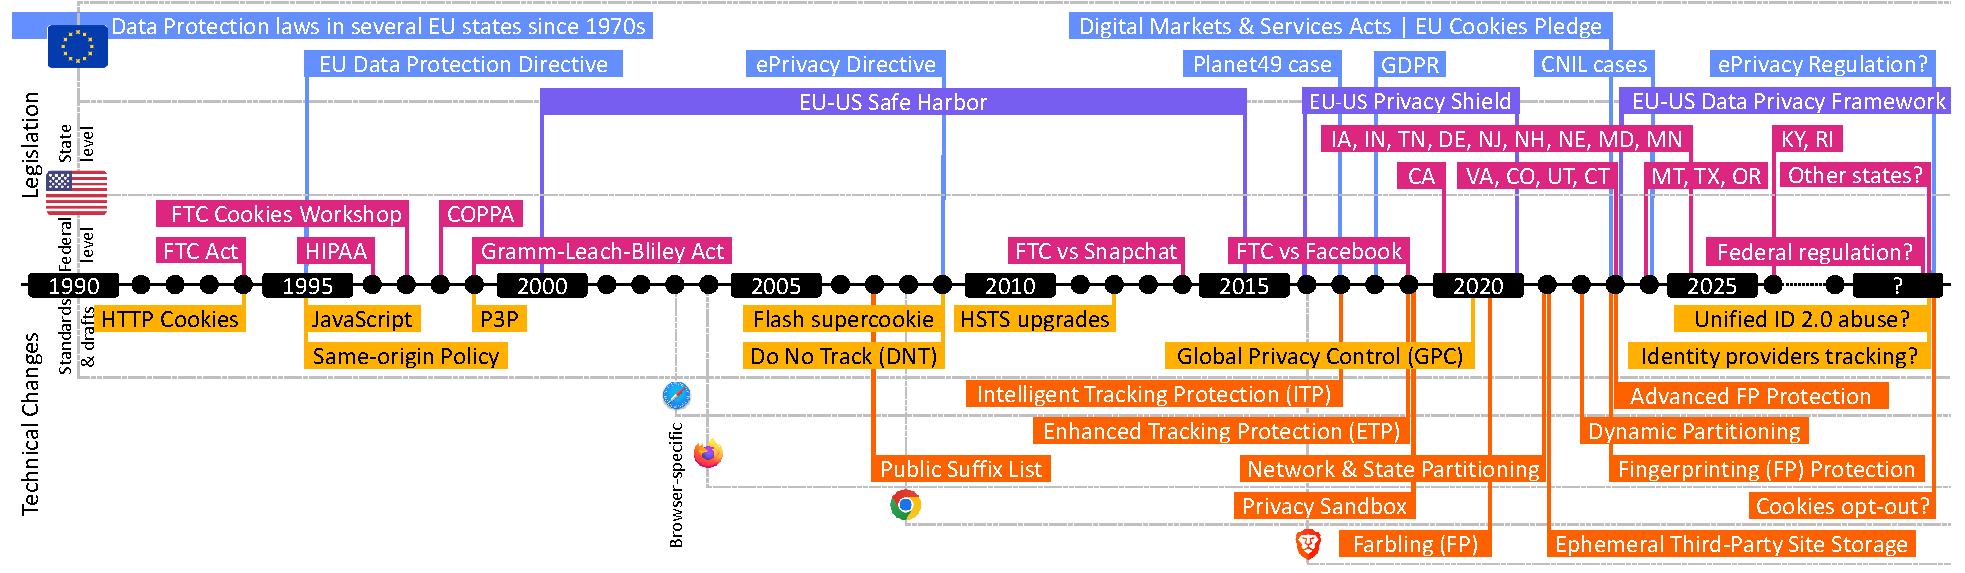
\includegraphics[width=\textwidth]{figures/timeline.pdf}
    \caption{Timeline of major technical and browser-specific changes with regulation overview in the EU and US.}
    \label{fig:timeline}
    \vspace{-4mm}
\end{figure*}